\documentclass[12pt]{emulateapj}
\newcommand{\beq}{\begin{equation}}
\newcommand{\eeq}{\end{equation}}
\newcommand{\hyd}    {{\rm H}}
\newcommand{\vobs}{v_{\rm obs}}
\newcommand{\hi}{H{\sc i}~}
\newcommand{\hii}{H{\sc ii}~}
\newcommand{\hia}{H{\sc i}}
\newcommand{\hiia}{H{\sc ii}}

\usepackage[colorlinks,urlcolor=blue,citecolor=blue,linkcolor=blue]{hyperref}
\usepackage{gensymb}
\usepackage{amsmath}
\usepackage{color}

\makeatletter
\setlength{\@fptop}{0pt}
\setlength{\@fpbot}{0pt}
\setlength{\@fpsep}{0pt}
\makeatother

\newcommand{\citei}[1]{\citeauthor{#1} \citeyear{#1}}
\newcommand{\unit}[1]{\textrm{ #1}}
\newcommand{\kms}{km ${\rm s^{-1}}$}
\newcommand{\kmsa}{km ${\rm s^{-1}}$}
\newcommand{\citeia}[2]{\citeauthor{#1}~(\citeyear{#1};~#2)}

\newcommand\reye{\mathrel{Re}}
\newcommand\reym{\mathrel{Rm}}

\renewcommand{\topfraction}{0.85}
\renewcommand{\textfraction}{0.1}
\renewcommand{\floatpagefraction}{0.75}

\begin{document}

\title{The Weakly Nonlinear Saturation of the Magnetorotational Instability}
\author{Clark, S.E.\altaffilmark{1}}
\author{Oishi, J.S. \altaffilmark{2,}\altaffilmark{3}}
\author{Mac Low, M.-M.\altaffilmark{1,}\altaffilmark{2}}
\altaffiltext{1}{Department of Astronomy, Columbia University, New York, NY} 
\altaffiltext{2}{Department of Astrophysics, American Museum of Natural History, New York, NY}
\altaffiltext{3}{Department of Physics, SUNY Farmingdale}


\begin{abstract}
The magnetorotational instability (MRI) is a fundamental process of accretion disk physics, but its saturation mechanism remains poorly understood. We present an analytic analysis of the nonideal MRI in the weakly nonlinear regime -- that is, when the MRI system is just unstable to its most unstable mode. 
\end{abstract}



\section{Introduction}

The magnetorotational instability (MRI) arises in a differentially rotating disk with a vertical magnetic field.

\section{Set-Up}

Our domain is designed to be relevant to the design of the Princeton Plasma Physics Laboratory (PPPL) MRI experiment. The experimental apparatus is tall, one of many attributes designed to mitigate the meridional flows introduced by the endcaps. We use periodic vertical boundary conditions. On the radial boundaries of our domain --  the inner and outer cylinders -- we apply no-slip, perfectly conducting boundary conditions.

\section{Weakly Nonlinear Analysis}

We solve the equations of non-ideal, axisymmetric, incompressible magnetized Taylor Couette flow. We solve the momentum equation:

\beq
\partial_t \mathbf{u} \, + \, \mathbf{u} \cdot \nabla \mathbf{u} \, = 
\eeq

$\, -\frac{1}{\rho}\nabla P \, - \, \nabla\Phi \, + \, \frac{1}{\rho} \left(\mathbf{J}\times\mathbf{B}\right) \, + \, \nu\nabla^2 \mathbf{u} \, - \, 2\mathbf{\Omega} \times \mathbf{u} \, - \, \mathbf{\Omega} \times \left(\mathbf{\Omega} \times \mathbf{r} \right)$


and the induction equation:

\beq
\partial_t \mathbf{B} = \nabla \times \left(\mathbf{u} \times \mathbf{B}\right) + \eta\nabla^2\mathbf{B}
\eeq

Subject to the magnetic solenoid and incompressibility constraints:

\beq
\nabla \cdot \mathbf{B} = 0
\eeq

\beq
\nabla \cdot \mathbf{u} = 0
\eeq

We perturb the fluid quantities with three-dimensional, axisymmetric perturbations. We nondimensionalize the equations according to [...]
The fluid symbols $\mathbf{u}$, $\mathbf{B}$, etc. will henceforth be used to refer to the perturbed quantities.

We define the flux function $A$ and streamfunction $\Psi$. These are scalar fields defined as the curl of the magnetic field and velocity, respectively, and so automatically satisfy our constraints.

$A$ is thus related to the magnetic field as

\beq
\mathbf{B} \, = \, \left[\begin{matrix}
\partial_zA \\
B_{y} \\
-\partial_xA \\
\end{matrix}\right],\eeq \\

and $\mathbf{\Psi}$ is defined analogously.

The perturbed, nondimensionalized equations which will be the focus of this equation are as follows:

Our final equation set is: 

\begin{multline}
\label{eqset1}
\partial_t \nabla^2 \Psi \, + \, J\left(\Psi, \nabla^2 \Psi\right) \, - \, 2 \partial_z u_{1y} \, = \\
\, \frac{2}{\beta} B_0 \partial_z \nabla^2 A \, + \, \frac{2}{\beta}J\left(A, \nabla^2 A \right) \, + \, \frac{1}{\reye}\nabla^4 \Psi
\end{multline}

\begin{multline}
\label{eqset2}
\partial_t u_{1y} \, + \, J\left(\Psi, u_{1y}\right) \, + \, \left(2 - q\right) \Omega_0 \partial_z \Psi \, = \\
\, \frac{2}{\beta}B_0\partial_z B_{1y} \, + \, \frac{2}{\beta} J\left(A, B_{1y}\right) \, + \, \frac{1}{\reye} \nabla^2 u_{1y}
\end{multline}

\begin{multline}
\label{eqset3}
\partial_t A \, = \, B_0 \partial_z \Psi \, + \, J\left(A, \Psi\right) \, + \, \frac{1}{\reym} \nabla^2 A
\end{multline}

\begin{multline}
\label{eqset4}
\partial_t B_{1y} \, = \, B_0 \partial_z u_{1y} \, + \, J\left(A, u_{1y}\right) \, - \, J\left(\Psi, B_{1y}\right) \, \\
+ \, \frac{1}{\reym} \nabla^2 B_{1y}  \, - \, q \Omega_0 \partial_z A
\end{multline}

Where $J$ is the Jacobian operator, 
\beq
J\left(f, g\right) \equiv \partial_z f\partial_x g - \partial_x f \partial_z g.
\eeq  

Note that working in terms of the flux function raises the order of the first momentum equation.

The weakly nonlinear regime is where the MRI system is nonlinearly unstable to only the most unstable mode of the linear solution. We find the marginal state, where most unstable linear MRI mode neither grows nor decays, for a given set of dimensionless parameters. 

$B_0$ appears in Equations \ref{eqset1} - \ref{eqset4} because it is the nondimensionalized background field strength. That is, $B = B_0 \equiv 1$. In order to study our system in the weakly nonlinear regime, we tune the background magnetic field down away from stability (recall that stronger vertical fields stabilize the MRI). We do so by substituting $B = B_0\left(1 - \epsilon^2\right)$. The degree of departure from the marginal state is measured by the small parameter $\epsilon$. An $\mathcal{O}\left(\epsilon^2\right)$ weakening of the background magnetic field destabilizes a band of wave modes with width of $\mathcal{O}\left(\epsilon\right)$, which interact nonlinearly.

The destabilizing substitution is made, and Equations \ref{eqset1} - \ref{eqset4} are rewritten such that the fluid variables are contained in a state vector $\mathbf{V} = \left[\Psi, u_y, A, B_y\right]^\mathrm{T}$. This yields the following system of equations.

\beq
\mathcal{D}\partial_t \mathbf{V} + \mathbf{N} = \mathcal{L} \mathbf{V} - \epsilon^2\partial_z\mathcal{X} \mathbf{V} - \epsilon^2 \partial_z^3 \mathcal{L}_3\mathbf{V}
\eeq

Where $\mathcal{L} \equiv \mathcal{L}_0 + \mathcal{L}_1\partial_z + \mathcal{L}_2\partial_z^2 + \mathcal{L}_3\partial_z^3 + \mathcal{L}_4\partial_z^4$ \\

And:

\beq
\mathcal{D} = \left[\begin{matrix}
\nabla^2 & 0 & 0 & 0 \\
0 & 1& 0 & 0 \\
0 & 0 & 1 & 0\\
0 & 0 & 0 & 1 \\
\end{matrix}\right]
\eeq

\beq
\mathcal{L}_0 = \left[\begin{matrix}
\frac{1}{\reye}\partial_x^4 & 0 & 0 & 0 \\
0 & \frac{1}{\reye}\partial_x^2 & 0 &0 \\
0 & 0 & \frac{1}{\reym}\partial_x^2 & 0 \\
0 & 0 & 0 & \frac{1}{\reym}\partial_x^2 \\ \end{matrix}\right]
\eeq

\beq
\mathcal{L}_1 = \left[\begin{matrix}
0 & 2 & \frac{2}{\beta}\partial_x^2 & 0 \\
(\Omega_0 - 2)q & 0 & 0 & \frac{2}{\beta} \\
1 & 0 & 0 & 0 \\
0 & 1 & -q\Omega_0 & 0 \\ \end{matrix}\right] 
\eeq

\beq
\mathcal{L}_2 = \left[\begin{matrix}
2\frac{1}{\reye} \partial_x^2 & 0 & 0 & 0 \\
0 & \frac{1}{\reye} & 0 & 0 \\
0 & 0 & \frac{1}{\reym} & 0 \\
0 & 0 & 0 & \frac{1}{\reym} \\ \end{matrix}\right]
\eeq

\beq
\mathcal{L}_3 = \left[\begin{matrix}
0 & 0 & \frac{2}{\beta} & 0 \\
0 & 0 & 0 & 0 \\
0 & 0 & 0 & 0 \\
0 & 0 & 0 & 0 \\ \end{matrix} \right]
\eeq

\beq
\mathcal{L}_4 = \left[\begin{matrix}
\frac{1}{\reye} & 0 & 0 & 0 \\
0 & 0 & 0 & 0 \\
0 & 0 & 0 & 0 \\
0 & 0 & 0 & 0 \\ \end{matrix}\right] 
\eeq

\beq
\mathcal{X} = \left[\begin{matrix}
0 & 0 & \frac{2}{\beta}\partial_x^2 & 0 \\
0 & 0 & 0 & \frac{2}{\beta} \\
1 & 0 & 0 & 0 \\
0 & 1 & 0 & 0 \\ \end{matrix} \right]. 
\eeq


We conduct a formal multiscale analysis. Our perturbations are characterized in terms of fast and slow-moving variables, in order to simultaneously track their evolution on fast and slow scales. The relative scalings of the fast and slow scales are determined as follows. When our four equations are linearized for axisymmetric perturbations of the form $e^{\sigma t + i k_x x + i k_z z}$, we can derive the linear dispersion relation, which is fourth order in $\sigma$. The fast and slow variables are then defined such that each of the temporal and spatial eigenvalues appear at the same lowest order in the linear dispersion relation. The scalings are: 

\beq
X \equiv \epsilon x,  \, \, Y \equiv \epsilon y, \, \, Z \equiv \epsilon z, \, \, T \equiv \epsilon^2 t
\eeq

Note that these are the same scalings as apply to Rayleigh-B\'enard convection and hydrodynamic Taylor Couette flow. Each operator is expanded to reflect these scalings -- for instance, $\partial_z$ becomes $\partial_z + \epsilon\partial_Z$. 

The multiple scale dependencies of our solution are encoded into an ansatz for the linear MRI solution at marginality,

\beq
\label{V1_ansatz}
\mathbf{V_1} = \alpha(T, Z) \mathbb{V}_{11}(x) e^{i k_c z} + c.c.,
\eeq

where $\alpha$ is a slowly-varying amplitude equation. The $x$ dependence is contained in $\mathbb{V}_{11}$, and must be solved for subject to the radial boundary conditions. The periodic vertical boundary conditions allow us to posit the $z$ dependence, where $k_c$ is the value of the vertical wavenumber at marginality. 

Because we investigate the system at marginality, where the growth rate $\sigma = 0$, the $\partial_t$ terms drop out. Thus after the multiscale expansion our system becomes

\begin{multline}
\label{multiscale_system}
\epsilon^2 \mathcal{D}\partial_T\mathbf{V} \, + \, \mathbf{N} \, = \, \mathcal{L}\mathbf{V} \, + \, \epsilon\widetilde{\mathcal{L}}_1\partial_Z\mathbf{V} \, + \, \epsilon^2\widetilde{\mathcal{L}}_2\partial_Z^2\mathbf{V} \, \\
 - \, \epsilon^2\partial_z\mathcal{X}\mathbf{V} \, - \, \epsilon^2\partial_z^3\mathcal{L}_3\mathbf{V} \, + \, \mathcal{O}(\epsilon^3)
\end{multline}

Where

\beq
\widetilde{\mathcal{L}}_1 = \mathcal{L}_1 + 2\mathcal{L}_2\partial_z + 3\mathcal{L}_3\partial_z^2 + 4\mathcal{L}_4\partial_z^3
\eeq

\beq
\widetilde{\mathcal{L}}_2 = \mathcal{L}_2 + 3\mathcal{L}_3\partial_z + 6\mathcal{L}_4\partial_z^2
\eeq


% perturbation expansion
The state vector is expanded in orders of $\epsilon$:

\beq
\label{pert_exp}
\mathbf{V} = \epsilon\mathbf{V_1} + \epsilon^2\mathbf{V_2} + \epsilon^3\mathbf{V_3} + ...
\eeq

Substituting Equation \ref{pert_exp} into Equation \ref{multiscale_system} yields the perturbed, expanded equations. We solve these successively in increasing orders of $\epsilon$.

To $\mathcal{O}(\epsilon)$, we have

\beq
\label{ordere}
\mathcal{L}\mathbf{V_1} = 0
\eeq

To $\mathcal{O}(\epsilon^2)$: 

\beq
\label{ordere2}
\mathcal{L}\mathbf{V_2} \, = \, \mathbf{N_2} \, - \, \widetilde{\mathcal{L}}_1 \partial_Z \mathbf{V_1}
\eeq

To $\mathcal{O}(\epsilon^3)$: 

\begin{multline}
\label{ordere3}
\mathcal{D}\partial_T \mathbf{V_1} \, + \, \mathbf{N_3} \, = \, \mathcal{L} \mathbf{V_3} \, + \, \widetilde{\mathcal{L}}_1\partial_Z\mathbf{V_2} \, + \, \widetilde{\mathcal{L}}_2\partial_Z^2\mathbf{V_1} \, \\
- \partial_Z\mathcal{X}\mathbf{V_1} \, - \partial_z^3\mathcal{L}_3\mathbf{V_1}
\end{multline}

The $\mathcal{O}(\epsilon)$ equation is the equation for the linear MRI at marginality. This is the equation that is solved to find the $\mathbb{V}_{11}$ component of Equation \ref{V1_ansatz}. 

The partial differential equations that comprise Equations \ref{ordere} to \ref{ordere3} are solved in succession subject to no-slip, perfectly conducting radial boundary conditions, defined as:

\beq
\Psi = \partial_x \Psi = u_y = A = \partial_x B_y = 0
\eeq

The practical advantage of our ansatz construction (Equation \ref{V1_ansatz}) is clear: the separable x-dependence means that the radial boundary conditions are solved in only one dimension. Thus our analytical framework is able to side-step many of the resolution issues faced by multidimensional simulations. We are able to resolve even significant structure in the boundary layers of our domain, because we need only resolve it in one dimension. We solve the radial component of each equation using the open source pseudospectral code Dedalus (Burns et al., in prep). We compute the radial components on a grid of Chebyshev polynomials, as is appropriate for bounded one-dimensional domains (e.g. CITE). 

We solve the system up to $\mathcal{O}(\epsilon^3)$ in order to close the solution at $\mathcal{O}(\epsilon^2)$. 

To find a bounded solution at each order, we eliminate secular terms -- terms which are resonant with solutions to the homogenous equation, and cause the solution to grow without bound. The elimination of secular terms requires enforcement of solvability criteria, which arise as a consequence of the Fredholm alternative (e.g. Guenther \& Lee 1988). The solvability criterion is found by forcing the inner product of the equation with its adjoint homogenous solution to be zero. For instance, Equation \ref{ordere2} contains a term $\widetilde{\mathcal{L}}_1 \partial_Z \mathbf{V_1}$ that is resonant with $e^{i k_c z}$. Because the adjoint homogenous equation

\beq
\mathcal{L}^\dagger \mathbf{V}^\dagger = 0
\eeq

has a nontrivial solution, the solvability criterion

\beq
\left< \mathbf{V}^\dagger \cdot \widetilde{\mathcal{L}}_1 \partial_Z \mathbf{V_1}\right> = 0 
\eeq

must be satisfied in order for Equation \ref{ordere2} to have a solution. In the above, 

\beq
\mathbf{V}^\dagger = \mathbb{V}^\dagger e^{iQz} + c.c.
\eeq

The elimination of this inner product must also be enforced the terms in Equation \ref{ordere3} that are resonant with $e^{i k_c z}$, yielding

\beq
\label{ampeq1}
a \partial_T \alpha \, + \, c \alpha \left|\alpha^2\right| \, + \, \widetilde{c} \alpha \partial_Z \beta \, = \, - b \partial_Z \alpha \, + \, h \partial_Z^2 \alpha \, + \, g i Q^3 \alpha
\eeq

Where

\begin{multline}
a \equiv \left< \mathbb{V}^\dagger \cdot \mathcal{D}\mathbb{V}^*_{11}\right> \\
c \equiv \left< \mathbb{V}^\dagger \cdot \mathbf{N}^*_{31}\right> \\
\widetilde{c} \equiv \left< \mathbb{V}^\dagger \cdot \widetilde{\mathbf{N}}^*_{31}\right> \\
b \equiv \left< \mathbb{V}^\dagger \cdot \left(\mathcal{X}\mathbb{V}_{11}\right)^* \right> \\
h \equiv \left< \mathbb{V}^\dagger \cdot \left(\widetilde{\mathcal{L}}_2\mathbb{V}_{11} \, - \, \widetilde{\mathcal{L}}_1\mathbb{V}_{21} \right)^* \right> \\
g \equiv \left< \mathbb{V}^\dagger \cdot \mathcal{L}_{3} \mathbb{V}_{11} \right> \\
\end{multline}

Equation \ref{ampeq1} is an amplitude equation -- a function of the slow variables $Z$ and $T$. We solve this initial value problem using Dedalus to obtain the asymptotic behavior of $\alpha$. This is the saturation amplitude.

\section{Results}

\begin{figure*}[h!]
\centering
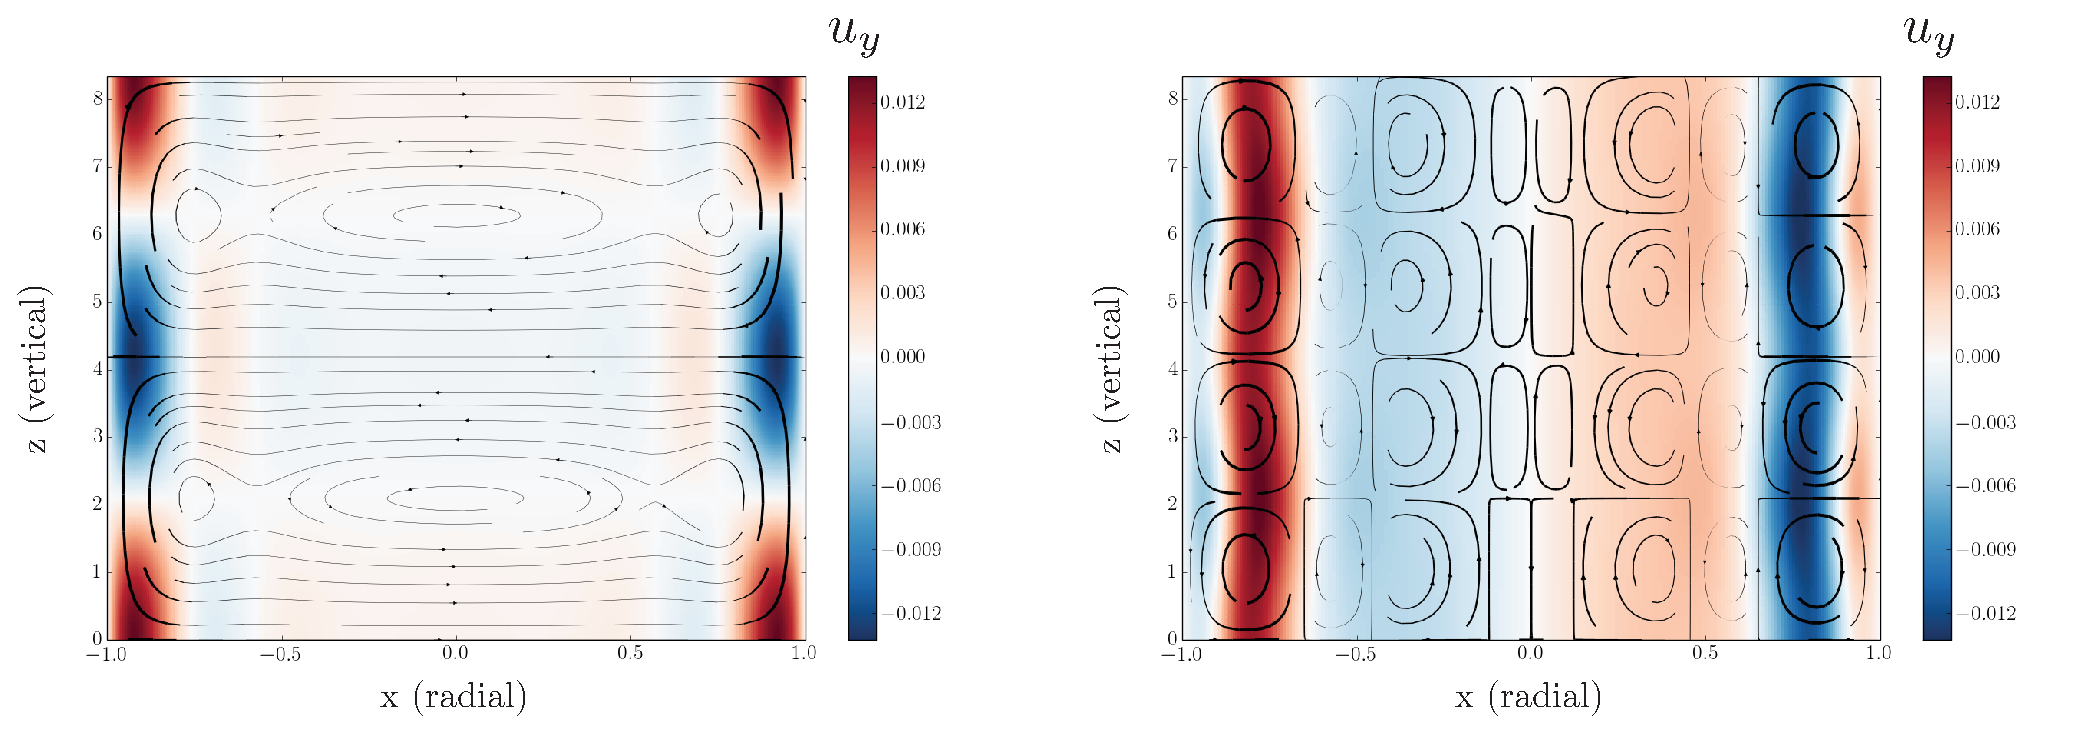
\includegraphics[scale=0.5]{twoorders_velocity.eps}
\caption{First order (left) and second order (right) velocity perturbations. Streamlines represent velocity in the vertical-radial plane, where thicker streamlines correspond to faster speeds. The colorbar represents azimuthal velocity.}
\end{figure*}

\section{Conclusions}



\end{document}
